\section{Visual Text Analysis Using \system}
\label{sec:system}
We now discuss various components of \system user interface and explain how these components enable users to perform various text data analysis and visualization tasks. The three key components of the interface are a Data View, a Chart View, and a Code Editor. \system also has a dropdown-style operations menu within it's menubar.
The operations menu allows users to use built-in text analysis and visualization operation. 

\stitle{Code Editor and Operations Menu.}
The Code Editor design (see Figure~\ref{fig:fe}C) is inspired by computational notebooks. 
However, the traditional notebooks are often criticised for their linear representation, making it difficult to explore visualizations and data and to maintain the context of the data analysis workflow~\cite{?}. The \system Code Editor only supports writing, editing, and executing scripts---visualizations and data tables are displayed separately in Chart View and Data View, respectively. The multi-view representation is intended to help users in more flexible exploration within the analytics session. Users can write scripts in the Code Editor in Python language. We also introduce a set of operators for analyzing and visualizing data using an algebra called \vta (discussed in Section~\ref{sec:vta}). The \vta commands are accesible via a Python library called \vital (also discussed in Section~\ref{sec:vta}).
Figure~\ref{fig:workflow} shows an example workflow written in \vital where a user first loads a review data, then cleans the ``review'' column within the dataset, featurizes the data, and finally, creates a bar chart visualization. We discuss how data and charts are generated and displayed in their corresponding views later.

\begin{figure}[!htb] 
%  \vspace{-10pt}
  \centering
  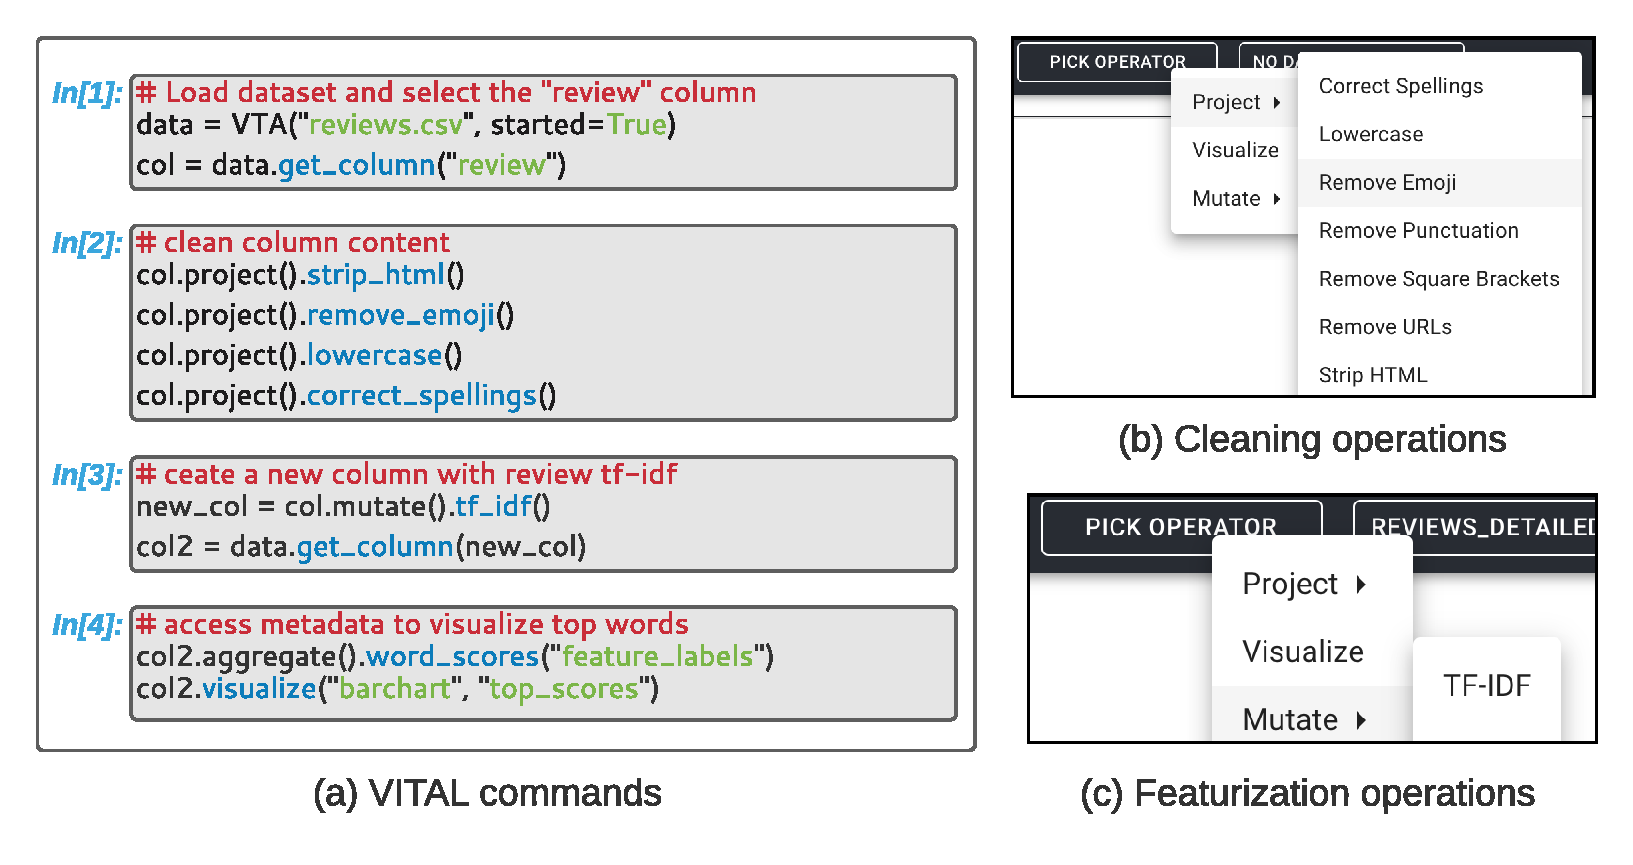
\includegraphics[width=\linewidth]{figures/vital.pdf}
  \caption{\small \system provides an API called \vital (visual interactive text analysis library) to enable users to run \vta operations within Notebook View. (a) An example usage of \vital. A user first loads a review data, then cleans the ``review'' column within the dataset, featurizes the data, and finally, creates a bar chart visualization. Instead of writing scripts, the user can also utilize the built-in (b) cleaning, (c) featurization, and visualization operations available via the drop-down menu. The \vital equivalences of the menu-driven operations are also interactively prompted to the user in Notebook View for improved accessibility and reuse. \label{fig:workflow}} 
  %\vspace{-20pt}
\end{figure}

Instead of writing \vital commands, users can also utilize the Operations Menu to execute built-in relevant analysis and visualization operations (see Figure~\ref{fig:workflow}a, ~\ref{fig:workflow}b, and ~\ref{fig:workflow}c). Other features in the Operations Menu involve uploading data and pre-trained models. However, the Code Editor provides more flexibility and a wider range of operations. For example, users cannot create custom operators from Operations Menu. The Code Editor supports these features. We show in Section~\ref{sec:vta} how users can write custom functions in Code Editor that become new operators in Operations Menu. 

\todo{Operations menu is interaction is added to Code Editor. Any metadata created becomes part of the operator view suggestion.}


\begin{figure}[!htb] 
%  \vspace{-10pt}
  \centering
  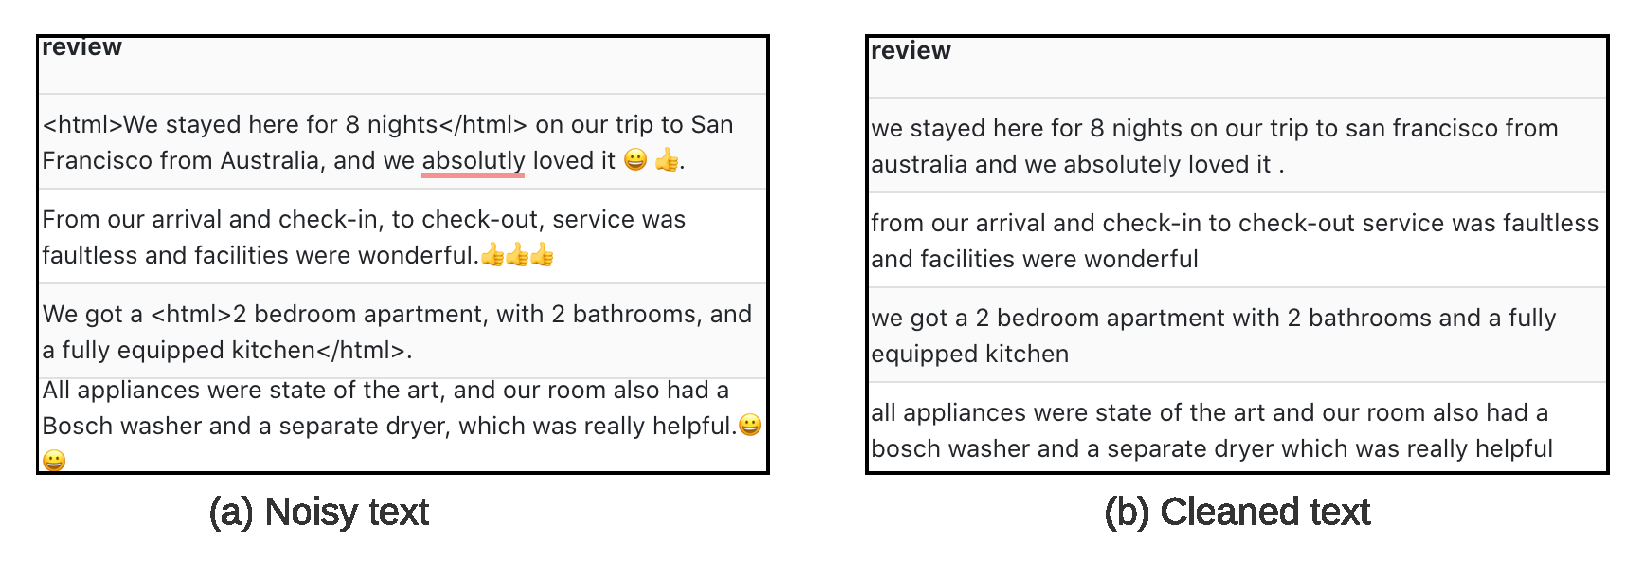
\includegraphics[width=\linewidth]{figures/data_view_clean.pdf}
  \caption{\small \system dynamically updates the effects of operations---run either via the interactive menu or from Notebook View---across relevant views of the data. (a) Noisy data with HTML tags, emojis, and typos in the ``review'' column. (b) After a user performs various cleaning operations on the `review'' column as shown in Figure~\ref{fig:workflow}, the changed column data is immediately displayed in Data View. \label{fig:dataview}} 
  %\vspace{-20pt}
\end{figure}

\stitle{Data View.}
Data View (see Figure~\ref{fig:fe}C) shows a tabular representation of the underlying data. Note that the underlying data structure in \system is a dataframe~\cite{rahman2020leam}. Data View is kept in sync with the dataframe---any changes made to the dataframe is immediately reflected in Data View. For example, in Figure~\ref{fig:dataview} when a user cleans the review column in the dataframe, the corresponding cleaned data is displayed in the Data View. Tehrefore, changes to the underlying data is immediately visible to the user. In traditional script-based systems like computation notebooks, users are required to explicitly specify a print operation to view and inspect data. \system currently supports one dataset per session. Whenever a new dataset is uploaded, the Data View is refreshed to display the new dataframe corresponding to that dataset. We discuss how to explore multiple datasets in Data View in Section~\ref{sec:discussion}. 
\todo{Future work, support filtering data in Table View which will create a new filtered the dataframe and pickle the original dataframe. Support multiple datasets.}

\stitle{Chart View.}
Text data analysis often involves generating visualizations like data distribution, aggregated summaries of attributes, to obtain further insights.
\system enables users to generate visualizations either from the Code Editor or Operations Menu and displays those visualizations in the Chart View. The charts are displayed within a carousel (see Figure~\ref{fig:fe}B). We create the visualizations using Vega-Lite~\cite{satyanarayan2016vega}. Figure~\ref{fig:chartview_interact}a shows a barchart corresponding to the \vital command in the fourth cell of the Code Editor in Figure~\ref{fig:workflow}a.

\todo{Fig 5 (a) is a bit confusing. It reads as if when a bar chart visualization is created, an arbitrary selection is also created and displayed by default.} 

\begin{figure}[!htb] 
%  \vspace{-10pt}
  \centering
  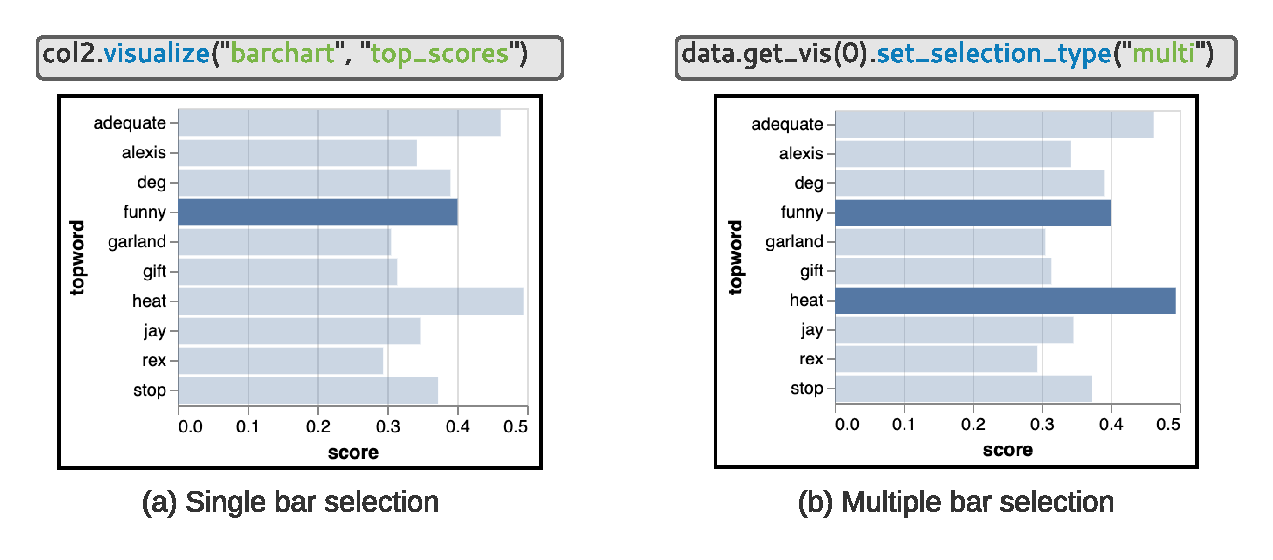
\includegraphics[width=\linewidth]{figures/chart_view_interact.pdf}
  \caption{\small \system enables a user to declaratively specify interactive selection (i.e. programmatic  mouse `clicking' or `brushing' effects) and view coordination. (a) A bar chart of top words in reviews ranked by their TF-IDF scores. The default selection  behavior is to select a single bar. (b) The user  dynamically specifies the \code{multi} selection type 
  to select multiple bars. We show the corresponding \vital command above each chart. \label{fig:chartview_interact}} 
  %\vspace{-20pt}
\end{figure}

However, Vega-Lite requires users to specify the visual encoding as well as supported interactions (\eg single or multple bar selection) before chart generation. \system enables users to specify such interactions dynamically using \vta view coordination algebra, \ie new interactions can be added on the fly even after the visualizations are created. For example, as shown in Figure~\ref{fig:chartview_interact}b, users can update the selection type of the barchart in Figure~\ref{fig:chartview_interact}a to enable multiple bar selection. Moreover, using the coordination algebra, users can also dynamically specify external coordinations between Data View and charts within the Chart View (see Section~\ref{sec:vta}). Vega-Lite currently does not provide a formal interaction grammar for external coordination. One alternative is to leverage the Vega Signals API~\cite{satyanarayan2015reactive} to enable coordination of Vega-Lite charts with external views.
However, unlike \system users cannot specify such coordination dynamically. For example, Figure~\ref{fig:chartview_coordinate} shows how users can enable coordination between the barchart, and scatterplots. Such dynamicity allows users to augment the visualizations instead of recreating charts and connect different views on demand to investigate data relationships. 

\begin{figure}[!htb] 
%  \vspace{-10pt}
  \centering
  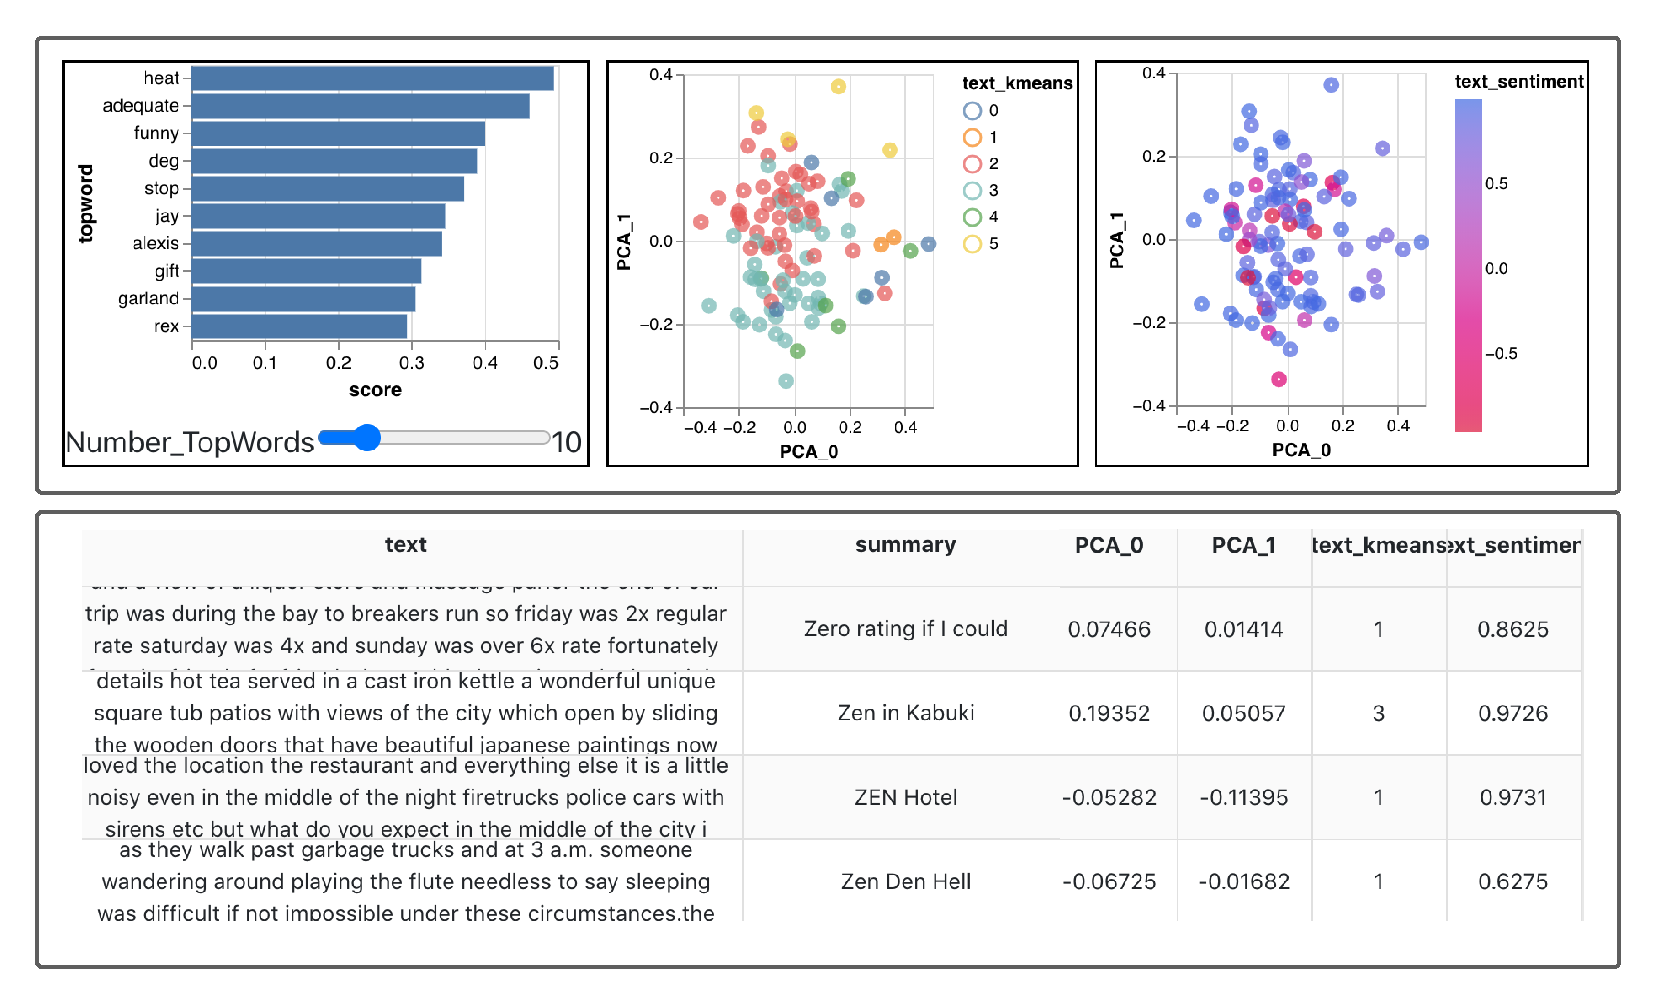
\includegraphics[width=\linewidth]{figures/chart_view.pdf}
  \caption{\small \todo{Draw figures} Example of dynamic coordination creation. The figure displays the barchart (generated in Figure~\ref{fig:chartview_interact}), a Scatterplot of reviews clustered using $k$-means clustering, and the corresponding data in Data View. To relate a word in the chart with reviews both in Data View and the scatterplot, the user issues a \vital command in Code Editor (see inset). Clicking a bar in the barchart filters reviews in Data View and highlights relevant reviews in the scatterplot. \label{fig:chartview_coordinate}} 
  %\vspace{-20pt}
\end{figure}






